%==================== Appendix.tex ====================

\clearpage
\thispagestyle{plain}

\begingroup
% เนื้อหาภาคผนวก: 16pt baseline ~19.2pt ตามสเปกเล่ม
\fontsize{16pt}{19.2pt}\selectfont
\justifying
\XeTeXlinebreakskip=0pt plus 1pt minus 0.5pt
\setlength{\parindent}{1.5cm}
\setlength{\parskip}{0pt}

\indent วิธีการใช้งานในส่วนของผู้จัดการประกวด เพื่อเป็นแนวทางในการใช้งานในส่วนที่ซับซ้อน และอาจทำให้สับสนในการใช้งานได้ จึงจัดทำคู่มือการใช้งานขึ้นมาเพื่ออำนวยความสะดวก

\vspace{\baselineskip}

\begin{figure}[h]
	\centering
	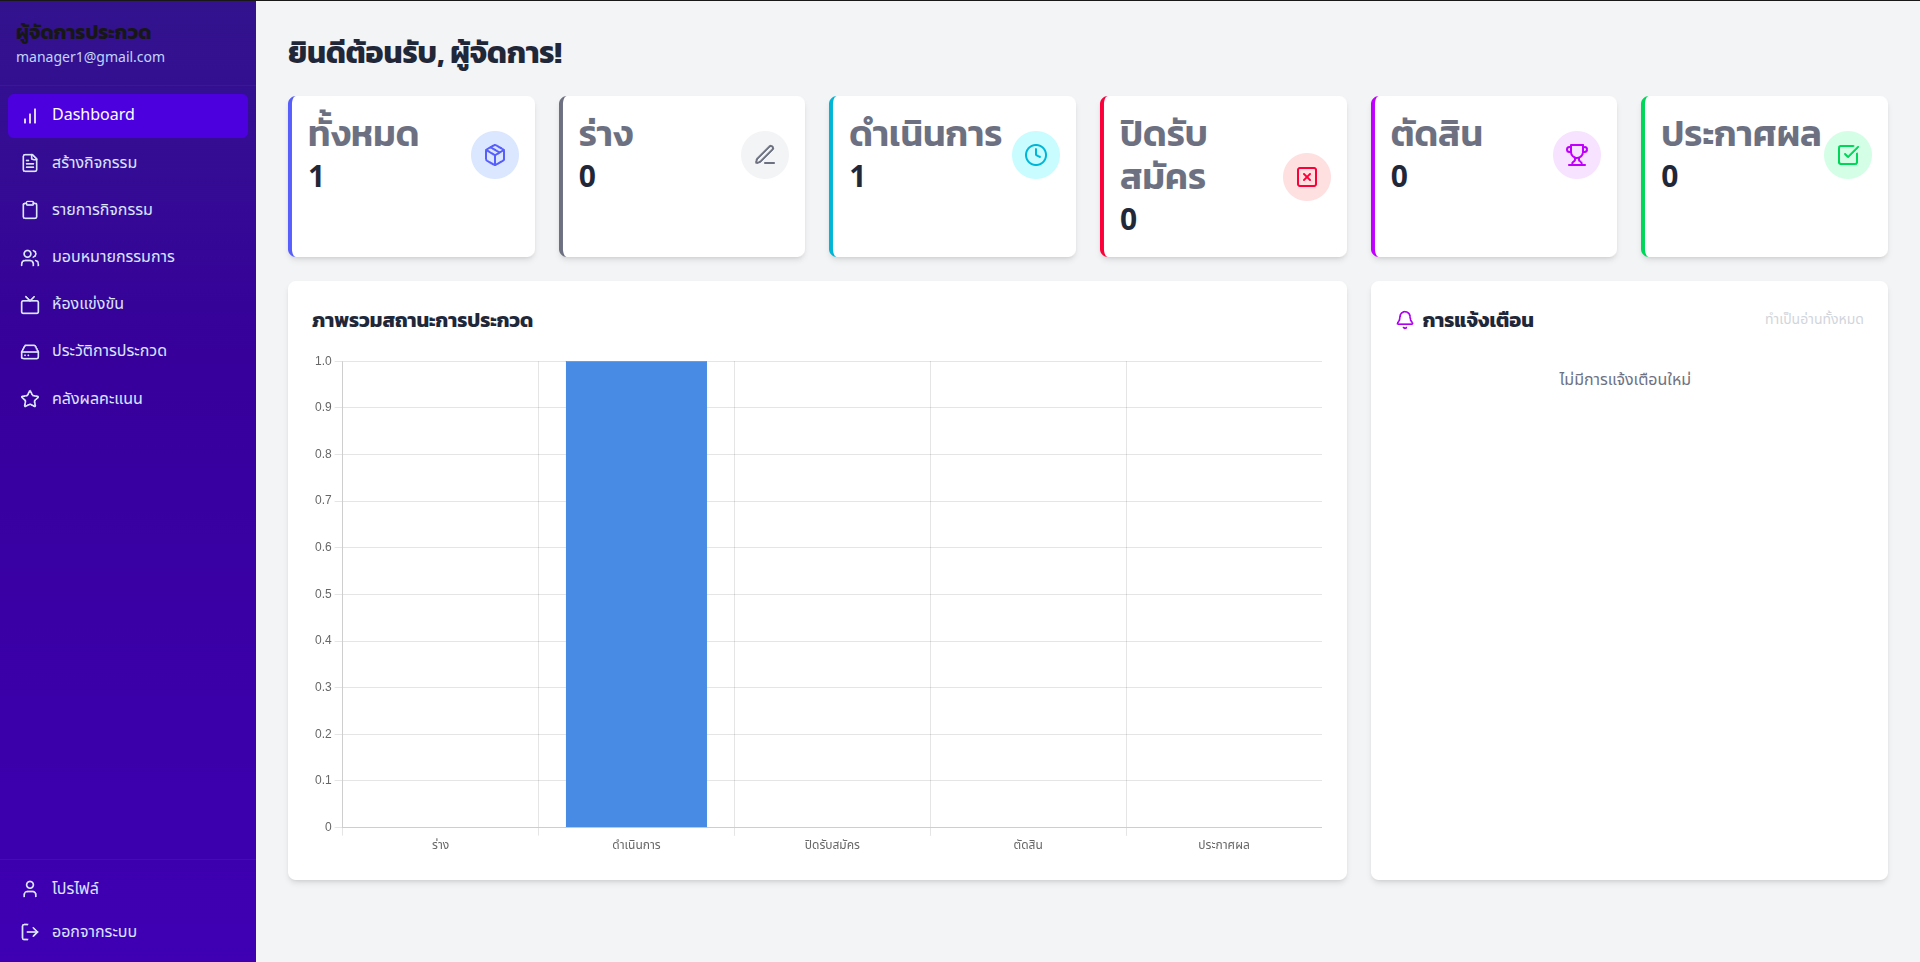
\includegraphics[width=0.8\linewidth]{MG1}
	\caption{หน้าแดชบอร์ดผู้จัดการ}
\end{figure}

\noindent{\bfseries\fontsize{16pt}{19.2pt}\selectfont วิธีใช้งานหน้าแดชบอร์ดผู้จัดการ}\par

\begin{sloppypar}
	\begin{enumerate}
		\item ดูภาพรวม สถิติการประกวด ผ่านการ์ดตัวเลข (ทั้งหมด/ร่าง/ดำเนินการ/ปิดรับสมัคร/ตัดสิน/ประกาศผล) และกราฟแท่ง “ภาพรวมสถานะการประกวด”
		\item พื้นที่ การแจ้งเตือน แสดงข้อความเหตุการณ์ล่าสุด สามารถ
		\begin{enumerate}
			\item กด ทำเป็นอ่านทั้งหมด เพื่อล้างรายการ
			\item คลิกลิงก์ ดูรายละเอียด (ถ้ามี) เพื่อไปยังหน้าที่เกี่ยวข้อง
		\end{enumerate}
		\item หากกำลังโหลดจะแสดง วงล้อหมุน; กรณีผิดพลาดจะแสดง ข้อความข้อผิดพลาด
		\item แดชบอร์ดจะแสดงชื่อผู้ใช้มุมบน (“ยินดีต้อนรับ, ผู้จัดการ/ชื่อจริง”)
	\end{enumerate}
\end{sloppypar}

\noindent{\bfseries\fontsize{16pt}{19.2pt}\selectfont ขั้นตอนใช้งาน}\par

\begin{sloppypar}
	\begin{enumerate}
		\item เข้าสู่หน้า แดชบอร์ดผู้จัดการ
		\item ดูการ์ดสรุปด้านบนเพื่อทราบจำนวนการประกวดในแต่ละสถานะอย่างรวดเร็ว
		\item เลื่อนลงดู กราฟแท่ง เพื่อเปรียบเทียบสัดส่วนสถานะต่าง ๆ ชัดเจน
		\item ที่กล่อง การแจ้งเตือน
		\begin{enumerate}
			\item อ่านข้อความล่าสุด และคลิก ดูรายละเอียด หากต้องการไปยังรายการนั้น
			\item ต้องการล้างทั้งหมด กด ทำเป็นอ่านทั้งหมด
			\item ต้องการลบทีละรายการ กดปุ่ม X ข้างข้อความ
		\end{enumerate}
		\item หากเห็นข้อความ กำลังโหลด… รอให้ข้อมูลแสดงผลครบ; ถ้าขึ้น ข้อผิดพลาด ให้รีเฟรชหน้าหรือกลับมาใหม่ภายหลัง
	\end{enumerate}
\end{sloppypar}

\vspace{\baselineskip}

\begin{figure}[h]
	\centering
	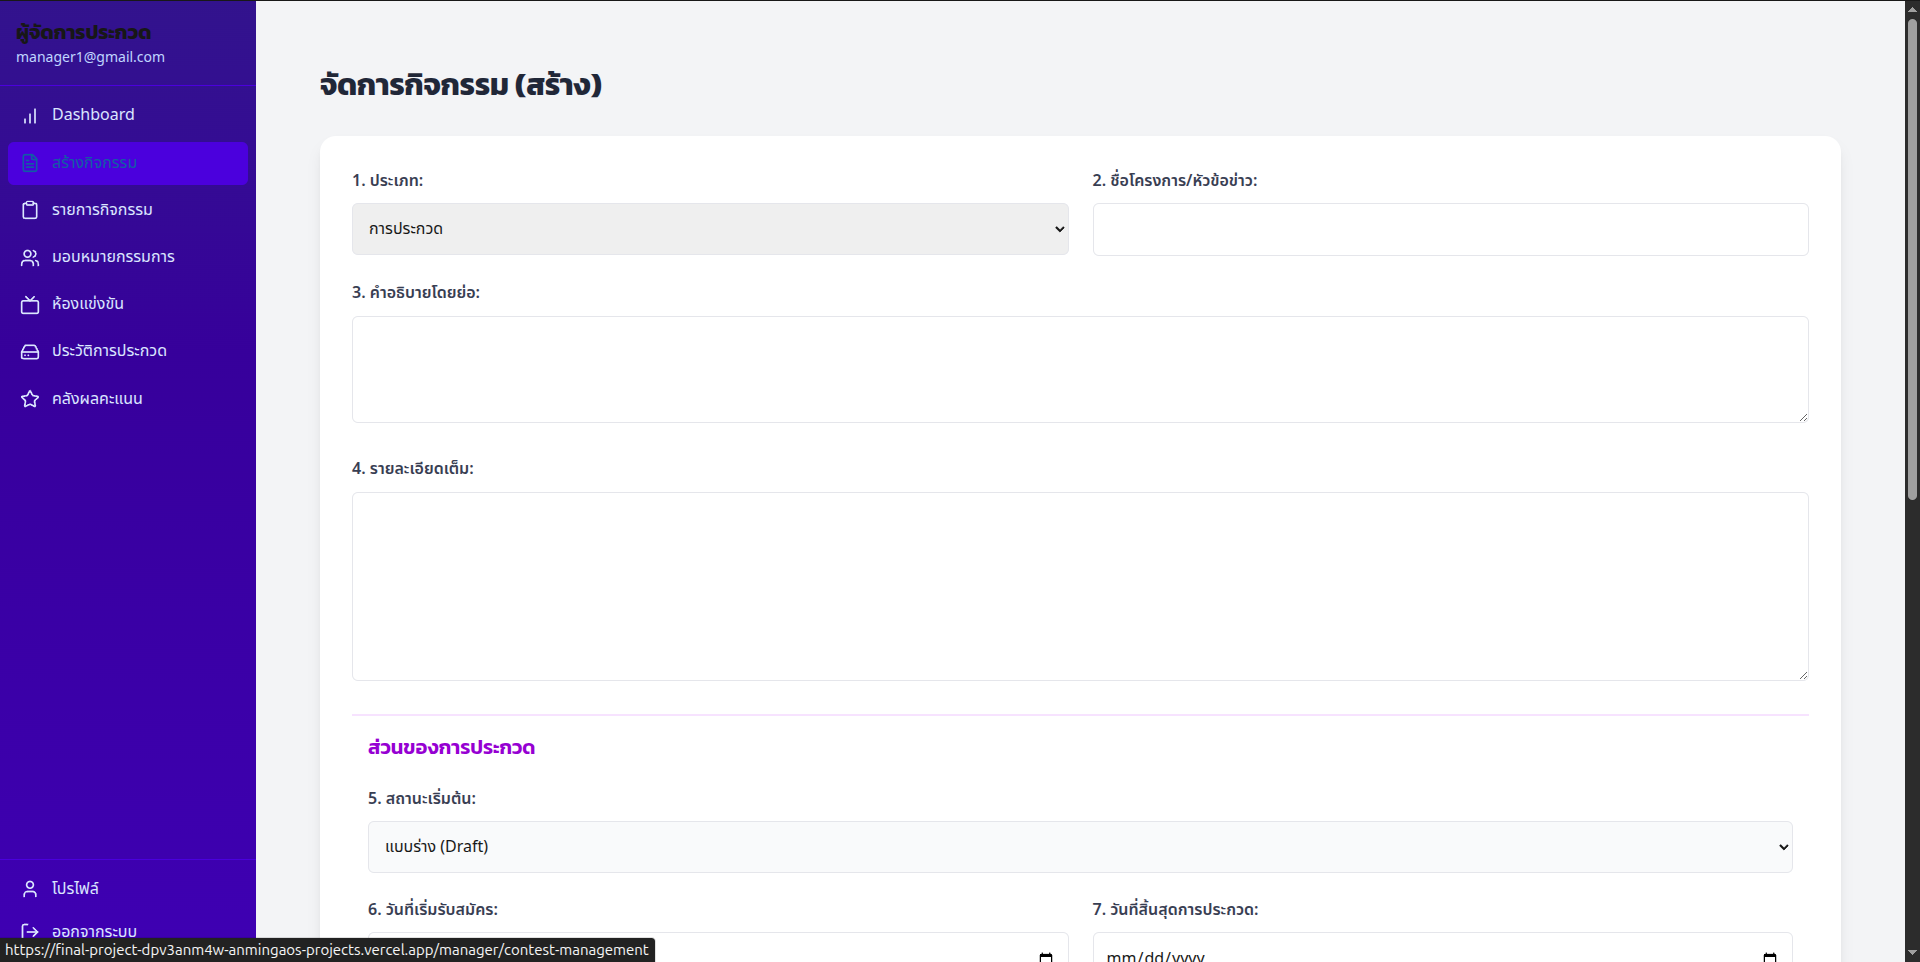
\includegraphics[width=0.8\linewidth]{MG2}
	\caption{หน้าจัดการกิจกรรม — สร้างการประกวด/ข่าว}
\end{figure}

\noindent{\bfseries\fontsize{16pt}{19.2pt}\selectfont วิธีใช้งานหน้าจัดการกิจกรรม — สร้างการประกวด/ข่าว}\par

\begin{sloppypar}
	\begin{enumerate}
		\item ใช้สำหรับ สร้างกิจกรรมใหม่ ได้ 2 ประเภท: การประกวด หรือ ข่าวสาร
		\item กรอกข้อมูลหลัก: ประเภท, ชื่อโครงการ/หัวข้อข่าว, คำอธิบายย่อ, รายละเอียดเต็ม (Rich Text)
		\item ไฟล์โปสเตอร์: อัปโหลดภาพ (PNG/JPG/WEBP) ขนาดไม่เกิน 5MB มีตัวอย่างแสดงและปุ่มลบ
		\item เมื่อเลือกประเภทเป็น การประกวด จะมีฟิลด์เพิ่มเติม
		\begin{enumerate}
			\item สถานะเริ่มต้น: แบบร่าง (Draft) หรือ เริ่มดำเนินการ (Published)
			\item วันที่เริ่มรับสมัคร / วันที่สิ้นสุด (ปฏิทินภาษาไทย, กันเลือกวันที่ย้อนหลัง/สิ้นสุดก่อนเริ่ม)
			\item ประเภทปลากัดที่เปิดรับ (เลือกได้ 1 ประเภท)
			\item คณะกรรมการ เลือกได้สูงสุด 3 คน (ค้นหาชื่อได้, รายการถูกกรองให้สัมพันธ์กับประเภทที่เลือก)
		\end{enumerate}
		\item ปุ่ม “บันทึกและสร้างกิจกรรม” จะส่งข้อมูลขึ้นระบบและแสดงสถานะกำลังทำงาน
	\end{enumerate}
\end{sloppypar}

\noindent{\bfseries\fontsize{16pt}{19.2pt}\selectfont ขั้นตอนใช้งาน}\par

\begin{sloppypar}
	\begin{enumerate}
		\item ไปที่หน้า จัดการกิจกรรม (สร้าง)
		\item เลือก ประเภท: การประกวด หรือ ข่าวสารทั่วไป/ประชาสัมพันธ์
		\item กรอก ชื่อโครงการ/หัวข้อข่าว, คำอธิบายย่อ, และพิมพ์ รายละเอียดเต็ม ในช่อง Rich Text
		\item อัปโหลด โปสเตอร์กิจกรรม (≤ 5MB)
		\begin{enumerate}
			\item ตรวจสอบตัวอย่างภาพได้ และกดปุ่ม ถังขยะ เพื่อลบ/อัปโหลดใหม่
		\end{enumerate}
		\item หากเลือกเป็น การประกวด
		\begin{enumerate}
			\item เลือก สถานะเริ่มต้น
			\item เลือก วันที่เริ่มรับสมัคร (ไม่น้อยกว่าวันปัจจุบัน) และ วันที่สิ้นสุด (ต้องไม่ก่อนวันเริ่ม)
			\item เลือก ประเภทปลากัดที่เปิดรับ (1 รายการ)
			\item ค้นหาและติ๊กเลือก คณะกรรมการ ได้สูงสุด 3 คน
		\end{enumerate}
		\item ตรวจทานความถูกต้อง แล้วกด “บันทึกและสร้างกิจกรรม”
		\begin{enumerate}
			\item ขณะส่ง ระบบจะแสดงไอคอนหมุน กำลังสร้างกิจกรรม...
			\item หากสำเร็จจะแจ้ง สร้างกิจกรรมสำเร็จ!; หากมีข้อผิดพลาดจะมีข้อความเตือนให้แก้ไข
		\end{enumerate}
	\end{enumerate}
\end{sloppypar}

\vspace{\baselineskip}

\begin{figure}[h]
	\centering
	\includegraphics[width=0.8\linewidth]{MG9}
	\caption{หน้าจัดการกิจกรรม — สร้างการประกวด/ข่าว}
\end{figure}

\noindent{\bfseries\fontsize{16pt}{19.2pt}\selectfont วิธีใช้งานหน้ารายการกิจกรรมทั้งหมด (แก้ไข/ลบ)}\par

\begin{sloppypar}
	\begin{enumerate}
		\item หน้านี้ใช้สำหรับดูรายการกิจกรรมทั้งหมดของผู้จัดการ (การประกวด/ข่าว) พร้อมโปสเตอร์ ชื่อ ช่วงวันเวลา และสถานะ (เฉพาะการประกวด)
		\item มีช่องค้นหาตามชื่อกิจกรรม และตัวกรองตามประเภท (การประกวด/ข่าว) และสถานะการประกวด (ร่าง/กำลังดำเนินการ/ปิดรับสมัคร/ตัดสิน/ประกาศผล/ยกเลิก)
		\item การ์ดกิจกรรมแต่ละใบมีปุ่ม ดูรายละเอียด (ไอคอนตา), แก้ไข (ดินสอ) และ ลบ (ถังขยะ)
		\item กด ดูรายละเอียด เพื่อเปิด Modal แสดงข้อมูลย่อ โปสเตอร์ วันเริ่ม–สิ้นสุด และรายชื่อกรรมการ (ถ้ามี)
		\item กด แก้ไข เพื่อเปิดหน้าต่างแก้ไขข้อมูลกิจกรรม (Edit Modal)
		\item กด ลบ เพื่อแสดงหน้าต่างยืนยันการลบ และยืนยันก่อนลบจริง
		\item ระหว่างดึงข้อมูลจะแสดงสถานะกำลังโหลด; หากเกิดข้อผิดพลาดจะแสดงข้อความแจ้งเตือน
	\end{enumerate}
\end{sloppypar}

\noindent{\bfseries\fontsize{16pt}{19.2pt}\selectfont ขั้นตอนใช้งาน}\par

\begin{sloppypar}
	\begin{enumerate}
		\item เปิดหน้า รายการกิจกรรมทั้งหมด (แก้ไข/ลบ)
		\item ใช้ช่องค้นหาเพื่อค้นหาตามชื่อ และ/หรือเลือกประเภทกิจกรรมที่ต้องการแสดง
		\item หากเลือกประเภทเป็น การประกวด ให้เลือกสถานะเพิ่มเติมเพื่อกรองผลลัพธ์
		\item ตรวจดูรายการที่แสดง (โปสเตอร์ ชื่อ วันเริ่ม–สิ้นสุด ป้ายสถานะสำหรับการประกวด)
		\item ดำเนินการกับรายการ:
		\begin{enumerate}
			\item กด ดูรายละเอียด เพื่อเปิด Modal และตรวจสอบข้อมูลย่อ/โปสเตอร์/กรรมการ
			\item กด แก้ไข เพื่อเปิด Edit Modal ปรับแก้ข้อมูล จากนั้นบันทึก
			\item กด ลบ เพื่อเปิดหน้าต่างยืนยัน ยืนยันการลบ เพื่อดำเนินการลบถาวร
		\end{enumerate}
		\item หากมีการแก้ไข/ลบสำเร็จ ระบบจะแจ้งผลและรีเฟรชรายการให้อัตโนมัติ
		\item หากไม่พบรายการที่ตรงเงื่อนไข จะปรากฏข้อความ ไม่พบรายการที่ตรงกับเงื่อนไข ให้ปรับการค้นหา/ตัวกรองใหม่
	\end{enumerate}
\end{sloppypar}

\vspace{\baselineskip}

\begin{figure}[h]
	\centering
	\includegraphics[width=0.8\linewidth]{MG10}
	\caption{หน้ามอบหมายกรรมการ}
\end{figure}

\noindent{\bfseries\fontsize{16pt}{19.2pt}\selectfont วิธีใช้งานหน้ามอบหมายกรรมการ}\par

\begin{sloppypar}
	\begin{enumerate}
		\item หน้านี้ใช้สำหรับมอบหมายกรรมการให้การประกวด โดยจำกัดจำนวนกรรมการสูงสุดต่อการประกวดไว้ที่ 3 คน
		\item ส่วนเลือกการประกวดจะแสดงการ์ดกิจกรรมที่สถานะเหมาะกับการมอบหมาย (ร่าง, กำลังดำเนินการ, ปิดรับสมัคร) พร้อมโปสเตอร์ ชื่อ และช่วงวันที่
		\item เมื่อเลือกการประกวดแล้ว จะแสดงรายชื่อกรรมการปัจจุบัน พร้อมสถานะตอบรับ เช่น รอดำเนินการ, ยอมรับแล้ว, ปฏิเสธแล้ว และมีปุ่มลบออกจากคณะกรรมการ
		\item ส่วนเลือกผู้เชี่ยวชาญเพิ่มเติมจะแสดงเฉพาะผู้เชี่ยวชาญที่ตรงกับประเภท/สาขาที่การประกวดเปิดรับ และสามารถค้นหาชื่อได้
		\item ผู้เชี่ยวชาญที่ถูกเลือกจะแสดงสถานะเลือกแล้ว และหากตรงความเชี่ยวชาญจะมีป้ายกำกับบอก
		\item ปุ่มล้างการเลือกทั้งหมดใช้เพื่อล้างรายชื่อผู้เชี่ยวชาญที่เลือกไว้ก่อนบันทึก
		\item ปุ่มบันทึกการมอบหมายใช้เพื่อยืนยันการเพิ่มกรรมการ ระบบจะตรวจสอบโควตาและแสดงสถานะกำลังมอบหมาย
		\item ระหว่างโหลดข้อมูลจะแสดงสถานะกำลังโหลด และหากเกิดข้อผิดพลาดจะแจ้งข้อความให้ทราบ
	\end{enumerate}
\end{sloppypar}

\noindent{\bfseries\fontsize{16pt}{19.2pt}\selectfont ขั้นตอนใช้งาน}\par

\begin{sloppypar}
	\begin{enumerate}
		\item เปิดหน้า มอบหมายกรรมการ
		\item เลือกการประกวดจากการ์ดรายการที่แสดง หากยังไม่พบรายการที่มอบหมายได้ ให้กลับไปสร้างหรือปรับสถานะการประกวดให้เหมาะสม
		\item ตรวจดูกรรมการปัจจุบันของการประกวด และลบรายชื่อที่ต้องการออกได้จากปุ่มลบ
		\item ในส่วนเลือกผู้เชี่ยวชาญเพิ่มเติม ให้พิมพ์ค้นหาชื่อหรือตรวจดูจากรายการที่ระบบคัดกรองให้ แล้วติ๊กเลือกผู้เชี่ยวชาญตามต้องการ
		\item สังเกตตัวนับโควตากรรมการ ว่าจำนวนรวมของที่มีอยู่แล้วและที่เลือกใหม่ไม่เกิน 3 คน
		\item หากต้องการเริ่มเลือกใหม่ทั้งหมด ให้กด ล้างการเลือกทั้งหมด
		\item เมื่อตรวจสอบถูกต้อง กด บันทึกการมอบหมาย ระบบจะเพิ่มกรรมการตามที่เลือกและรีเฟรชข้อมูล
		\item หากต้องการลบกรรมการภายหลัง ให้เลือกการประกวดเดิม กดลบที่รายชื่อนั้น ระบบจะลบและส่งการแจ้งเตือนให้ผู้เชี่ยวชาญ
	\end{enumerate}
\end{sloppypar}

\newpage

\vspace{\baselineskip}

\begin{figure}[h]
	\centering
	\includegraphics[width=0.8\linewidth]{MG11}
	\caption{หน้าห้องจัดการแข่งขัน}
\end{figure}

\noindent{\bfseries\fontsize{16pt}{19.2pt}\selectfont วิธีใช้งานหน้าห้องจัดการแข่งขัน}\par

\begin{sloppypar}
	\begin{enumerate}
		\item ใช้สำหรับบริหารการประกวดแบบเรียลไทม์: เลือกเวทีที่กำลังดำเนินการ ดู/คัดกรองรายชื่อผู้สมัคร ตรวจสถานะ AI ความคืบหน้าการให้คะแนน อนุมัติ/ปฏิเสธแบบเดี่ยวหรือหลายรายการ และเปลี่ยนสถานะการประกวดจนถึงประกาศผล
		\item การ์ดการแข่งขันแต่ละรายการแสดง โปสเตอร์ ชื่อ ช่วงวัน สถานะปัจจุบัน จำนวนกรรมการที่ตอบรับ และจำนวนผู้สมัคร คลิกการ์ดเพื่อเข้าสู่แดชบอร์ดของเวทีนั้น
		\item แถบสรุปบนแดชบอร์ดแสดงผู้สมัครทั้งหมด (นับคน) จำนวนปลากัด รวมถึงจำนวนตามสถานะ: รออนุมัติ อนุมัติแล้ว ประเมินแล้ว ปฏิเสธ และจำนวนกรรมการ
		\item ปุ่มจัดการสถานะการประกวด (มุมขวาบนของแดชบอร์ด) จะเปลี่ยนไปตามสถานะ: ปิดรับสมัคร  เริ่มการตัดสิน  คำนวณและประกาศผล
		\item ระหว่างสถานะ “ตัดสิน” จะแสดงความคืบหน้าการให้คะแนน: จำนวนกรรมการที่ตอบรับ จำนวนงานที่ครบทุกกรรมการ และเปอร์เซ็นต์ความครอบคลุมเฉลี่ย พร้อมปุ่มรีเฟรช
		\item ตารางรายชื่อผู้สมัครสามารถคัดกรองตามสถานะ (ทั้งหมด/รออนุมัติ/อนุมัติแล้ว/ประเมินแล้ว/ปฏิเสธ) และกรองย่อยด้วยสถานะ AI (ตรง/ไม่ตรง/ยังไม่มั่นใจ)
		\item สถานะ AI ต่อแถวแสดงเป็นป้ายสี: ตรง, ไม่ตรง, ยังไม่มั่นใจ และหากไม่ตรง สามารถเปิดดูรายละเอียดประเภทที่อนุญาตของเวทีได้
		\item แถวผู้สมัครมีปุ่มจัดการอย่างรวดเร็ว: ดูรายละเอียด อนุมัติ ปฏิเสธ (หรือยกเลิกการอนุมัติ), เปิดดูคะแนนกรรมการ รวมถึงกล่องติ๊กเพื่อทำรายการแบบกลุ่ม
		\item ในหน้า “ดูรายละเอียดผู้สมัคร” มีปุ่มให้ AI วิเคราะห์ภาพแรกของผลงานเพื่อช่วยพิจารณาความตรงประเภท พร้อมคำแนะนำให้ อนุมัติ/ตรวจเพิ่ม
		\item เมื่ออยู่ในแท็บ “ประเมินแล้ว” สามารถอนุมัติผลคะแนนแบบหลายรายการได้ในครั้งเดียว
	\end{enumerate}
\end{sloppypar}

\noindent{\bfseries\fontsize{16pt}{19.2pt}\selectfont ขั้นตอนใช้งาน}\par

\begin{sloppypar}
	\begin{enumerate}
		\item เข้าเมนู ห้องจัดการแข่งขัน แล้วเลือกการประกวดที่ต้องการบริหารโดยคลิกการ์ดของเวทีนั้น
		\item ตรวจสอบสถานะปัจจุบันของการประกวดในแถบด้านบน หากพร้อม
		\begin{enumerate}
			\item จาก กำลังดำเนินการ เลือก ปิดรับสมัคร
			\item จาก ปิดรับสมัคร เลือก เริ่มการตัดสิน เพื่อให้กรรมการเริ่มให้คะแนน
			\item จาก ตัดสิน เมื่อคะแนนครบ เลือก คำนวณและประกาศผล
		\end{enumerate}
		\item ใช้การ์ดสถิติเลือกมุมมอง เช่น รออนุมัติ/อนุมัติแล้ว/ประเมินแล้ว/ปฏิเสธ หรือดูรายชื่อกรรมการ
		\item ในมุมมองรายชื่อผู้สมัคร
		\begin{enumerate}
			\item เลือกกรองสถานะหลัก (เช่น รออนุมัติ) และถ้าต้องการให้แคบผลลัพธ์ยิ่งขึ้น ให้เลือกกรองสถานะ AI (ทั้งหมด/ตรง/ไม่ตรง/ยังไม่มั่นใจ)
			\item ติ๊กเลือกหลายรายการเพื่อทำงานแบบกลุ่ม แล้วกด อนุมัติที่เลือก / ปฏิเสธที่เลือก หรือในมุมมอง “ประเมินแล้ว” ให้กด อนุมัติผลคะแนนที่เลือก
			\item จัดการรายเดี่ยวด้วยปุ่มบนแถว: ดูรายละเอียด อนุมัติ ปฏิเสธ (หรือยกเลิกการอนุมัติ) และ ดูคะแนน
		\end{enumerate}
		\item เมื่อต้องการใช้ AI ช่วยตรวจประเภท
		\begin{enumerate}
			\item กด ดูรายละเอียด บนแถวผู้สมัคร
			\item กด วิเคราะห์ด้วย AI ระบบจะแสดงผลการทำนาย ความมั่นใจ และคำแนะนำ (อนุมัติ/ตรวจเพิ่ม)
		\end{enumerate}
		\item ระหว่างสถานะ “ตัดสิน” ตรวจความคืบหน้าการให้คะแนนจากแถบสรุป และกด รีเฟรช เพื่ออัปเดตล่าสุด
		\item เมื่อคะแนนครบถ้วน ให้กด คำนวณและประกาศผล ระบบจะยืนยันก่อนดำเนินการและปิดขั้นตอนของเวทีนั้น
	\end{enumerate}
\end{sloppypar}

\newpage

\begin{figure}[h]
	\centering
	\includegraphics[width=0.8\linewidth]{MG12}
	\caption{หน้าประวัติและผลการประกวด}
\end{figure}

\noindent{\bfseries\fontsize{16pt}{19.2pt}\selectfont วิธีใช้งานหน้าประวัติและผลการประกวด}\par

\begin{sloppypar}
	\begin{enumerate}
		\item ใช้สำหรับดูประวัติการแข่งขันที่ผ่านมา พร้อมสรุปผลผู้ชนะและคะแนนเรียงลำดับจากมากไปน้อย
		\item มีช่องค้นหาเพื่อกรองรายการตามชื่อการประกวดในอดีตแบบเรียลไทม์
		\item การ์ดแต่ละรายการแสดงชื่อการประกวด วันที่สิ้นสุด สถานะล่าสุด และไฮไลต์ผู้ชนะ (เมื่อสถานะเป็น “ประกาศผล”)
		\item ปุ่ม ดูผลสรุป จะเปิดหน้าต่างสรุปผล แสดงอันดับที่ 1–3 พร้อมชื่อปลา เจ้าของ และคะแนนรวม
		\item ระหว่างโหลดข้อมูลจะแสดงสถานะกำลังโหลด และหากเกิดข้อผิดพลาดจะแสดงข้อความแจ้งเตือน
		\item หากไม่พบรายการตามคำค้นหาหรือยังไม่มีประวัติ จะแสดงข้อความบอกสถานะให้ทราบ
	\end{enumerate}
\end{sloppypar}

\noindent{\bfseries\fontsize{16pt}{19.2pt}\selectfont ขั้นตอนใช้งาน}\par

\begin{sloppypar}
	\begin{enumerate}
		\item เข้าเมนู ประวัติและผลการประกวด
		\item พิมพ์คำค้นในช่อง ค้นหาชื่อการประกวดในอดีต... เพื่อกรองรายการ (ไม่พิมพ์ก็เห็นทั้งหมด)
		\item ดูสรุปในแต่ละการ์ด: วันที่สิ้นสุด สถานะ และผู้ชนะ (ถ้ามี)
		\item คลิกปุ่ม ดูผลสรุป ของรายการที่สนใจ
		\item ในหน้าต่างสรุปผล ตรวจดูอันดับ 1–3 พร้อมคะแนนรวมและข้อมูลเจ้าของปลา
		\item ปิดหน้าต่างสรุปเมื่อเสร็จสิ้น หรือเลือกดูรายการอื่น ๆ ต่อได้ตามต้องการ
	\end{enumerate}
\end{sloppypar}

\clearpage